\chapter{Implementasi dan Pengujian}
Bab ini akan berisi tentang implementasi perangkat lunak serta pengujian pada perangkat lunak tersebut. Hasil dari pengujian akan digunakan untuk menarik kesimpulan. 

\section{Implementasi}
Perangkat lunak akan diimplementasikan menjadi sebuah program dengan menggunakan bahasa Java. Rancangan antarmuka yang telah dijelaskan pada Bab \ref{perancangan_antarmuka}, telah berhasil diimplementasikan dan dapat dilihat pada gambar-gambar di bawah ini.

\begin{figure}[H]
	\centering
	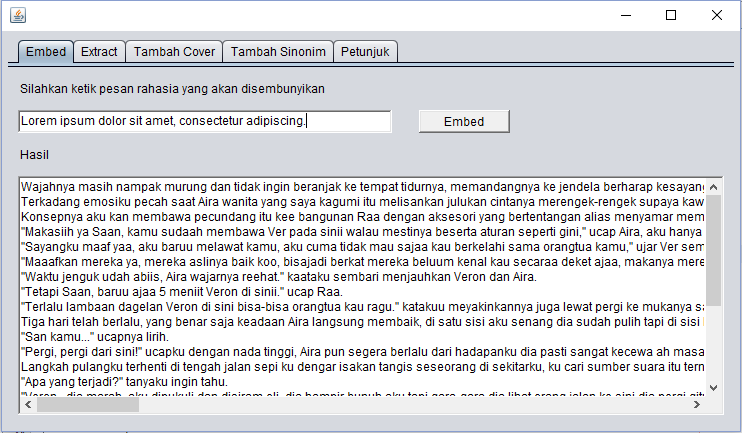
\includegraphics[scale=0.8]{Gambar/ui-embed}
	\caption{Tampilan \textit{tab Embed}} 
	\label{fig:ui-embed}
\end{figure}

\begin{figure}[H]
	\centering
	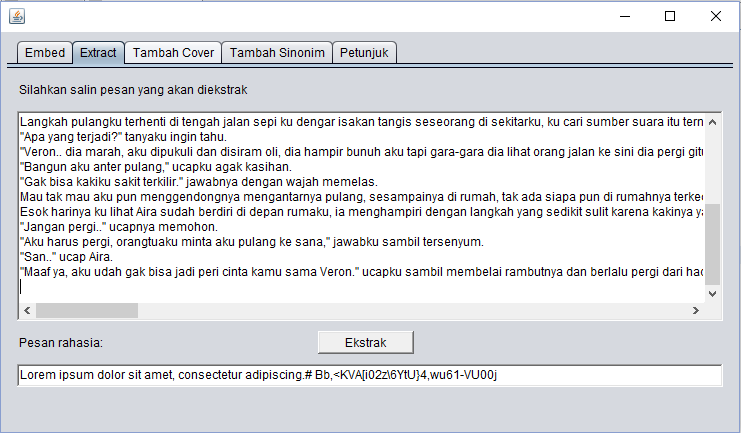
\includegraphics[scale=0.8]{Gambar/ui-extract}
	\caption{Tampilan \textit{tab Extract}} 
	\label{fig:ui-extract}
\end{figure}

Gambar \ref{fig:ui-extract} menunjukkan bahwa ada karakter '\#' yang memberitahu penerima bahwa pesan rahasia telah berakhir, seperti yang telah dijelaskan pada Bab \ref{algoritma}.

\begin{figure}[H]
	\centering
	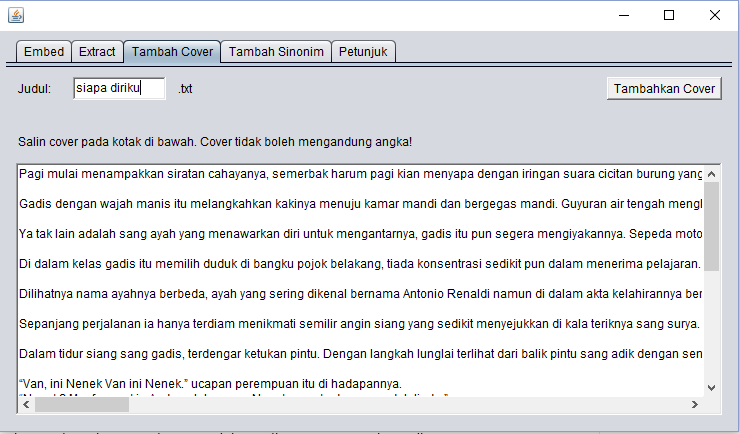
\includegraphics[scale=0.8]{Gambar/ui-tambah-cover}
	\caption{Tampilan \textit{tab Tambah Cover}} 
	\label{fig:ui-tambah-cover}
\end{figure}

\begin{figure}[H]
	\centering
	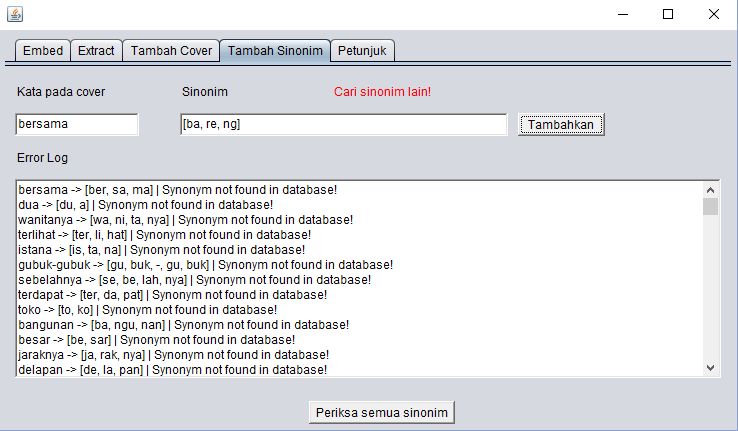
\includegraphics[scale=0.8]{Gambar/ui-tambah-sinonim}
	\caption{Tampilan \textit{tab Tambah Sinonim}} 
	\label{fig:ui-tambah-sinonim}
\end{figure}

Gambar \ref{fig:ui-tambah-sinonim} merupakan contoh saat pengirim memasukkan pasangan kata dan sinonim yang memiliki \textit{c}(\textit{w}) yang memiliki nilai yang sama. Seperti yang telah dijelaskan pada Bab \ref{perancangan_antarmuka}, jika penambahan sinonim gagal, \textit{textbox} sinonim akan diisi dengan hasil pemenggalan kata oleh perangkat lunak. Hal ini dilakukan untuk memberitahu pengirim bagaimana perangkat lunak memenggal kata tersebut. Pemenggalan kata yang dilakukan oleh perangkat lunak tidak sempurna, namun hal ini tidak menjadi masalah karena yang terpenting pemenggalan katanya konsisten.

\begin{figure}[H]
	\centering
	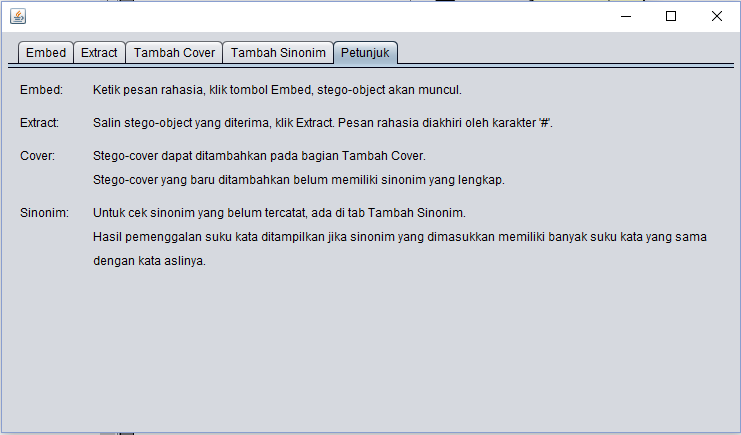
\includegraphics[scale=0.8]{Gambar/ui-petunjuk}
	\caption{Tampilan \textit{tab Petunjuk}} 
	\label{fig:ui-petunjuk}
\end{figure}

\section{Pengujian}
Pengujian yang dilakukan adalah pengujian fungsional dan pengujian eksperimental. Pengujian ini dilakukan untuk memeriksa apakah perangkat lunak yang dibuat telah berfungsi dengan baik. Hasil pengujian ini juga akan dipakai untuk menarik kesimpulan pada bab terakhir.

\subsection{Pengujian Fungsional}
Pengujian fungsional dilakukan untuk memeriksa apakah perangkat lunak memberikan reaksi yang seharusnya terhadap aksi dari pengguna perangkat lunak. Pengujian ini dilakukan pada sistem operasi Windows. Terdapat beberapa tes kasus yang diujikan, untuk lengkapnya dapat dilihat pada Tabel \ref{table-fungsional}.\\

\begin{table}[H]
\label{table-fungsional}
\centering
\caption{Tabel Pengujian Fungsional}
\begin{tabular}{|p{0.3cm} | p{4.5cm} | p{7cm} | p{1.5cm} |}\hline
No. & Aksi & Reaksi seharusnya & Hasil\\
\hline
1 & Pengguna mengetikkan pesan rahasia lalu menekan tombol Embed & Perangkat lunak menampilkan \textit{stego-cover} & Sesuai\\
2 & Pengguna memasukkan \textit{stego-object} lalu menekan tombol Extract & Perangkat lunak menampilkan pesan rahasia, karakter '\#' menandakan pesan rahasia telah berakhir & Sesuai\\
3 & Pengguna menambahkan \textit{stego-cover} & Perangkat lunak membuat \textit{file stego-cover} yang baru dan mendaftarkannya pada \textit{stego-cover list} & Sesuai\\
4 & Pengguna menambahkan sinonim & Perangkat lunak menambahkan sinonim ke kamus sinonim & Sesuai\\
5 & Pengguna memeriksa semua sinonim & Perangkat lunak menampilkan kata-kata yang sinonimnya tidak terdaftar pada kamus sinonim & Sesuai\\
\hline
\end{tabular}
\end{table}

\subsection{Pengujian Eksperimental}
Pengujian eksperimental ini dilakukan untuk menguji respon perangkat lunak terhadap beberapa kemungkinan yang dilakukan pengguna pada perangkat lunak.

\begin{table}[H]
\label{table-eksperimental}
\centering
\caption{Tabel Pengujian Eksperimental}
\begin{tabular}{|p{0.3cm} | p{5.5cm} | p{7.5cm} |}\hline
No. & Aksi & Reaksi \\
\hline
1 & Pengguna memasukkan pesan rahasia dengan ukuran yang tidak bisa ditampung \textit{stego-cover} & Perangkat lunak tidak mengeksekusi proses \textit{embed}. Muncul peringatan bahwa pesan rahasia melebihi kapasitas yang ada\\
2 & Pengguna menekan tombol \textit{embed}, namun \textit{stego-cover} belum memiliki sinonim yang lengkap & Perangkat lunak menampilkan kata apa saja yang belum terdaftar sinonimnya\\
3 & Pengguna memasukkan teks sembarang (bukan \textit{stego-object}) & Perangkat lunak mengeksekusi proses \textit{extract}, namun pesan yang diekstraksi tidak memiliki arti\\
4 & Pengguna menambahkan \textit{stego-cover} tanpa memasukkan nama \textit{file} & Muncul peringatan bahwa nama \textit{file} belum diisi\\
5 & Pengguna menambahkan \textit{stego-cover} dengan nama yang telah ada sebelumnya & Muncul peringatan bahwa nama \textit{file} telah dipakai\\
6 & Pengguna menambahkan sinonim dengan nilai \textit{c}(\textit{w}) yang sama dengan katanya & Muncul peringatan untuk mencari sinonim lain dan ditampilkan hasil pemenggalan sinonim yang dimasukkan pengguna\\
\hline
\end{tabular}
\end{table}